\documentclass[journal]{vgtc}                % final (journal style)
%\documentclass[review,journal]{vgtc}         % review (journal style)
%\documentclass[widereview]{vgtc}             % wide-spaced review
%\documentclass[preprint,journal]{vgtc}       % preprint (journal style)
%\documentclass[electronic,journal]{vgtc}     % electronic version, journal

%% Uncomment one of the lines above depending on where your paper is
%% in the conference process. ``review'' and ``widereview'' are for review
%% submission, ``preprint'' is for pre-publication, and the final version
%% doesn't use a specific qualifier. Further, ``electronic'' includes
%% hyperreferences for more convenient online viewing.

%% Please use one of the ``review'' options in combination with the
%% assigned online id (see below) ONLY if your paper uses a double blind
%% review process. Some conferences, like IEEE Vis and InfoVis, have NOT
%% in the past.

%% Please note that the use of figures other than the optional teaser is not permitted on the first page
%% of the journal version.  Figures should begin on the second page and be
%% in CMYK or Grey scale format, otherwise, colour shifting may occur
%% during the printing process.  Papers submitted with figures other than the optional teaser on the
%% first page will be refused.

%% These three lines bring in essential packages: ``mathptmx'' for Type 1
%% typefaces, ``graphicx'' for inclusion of EPS figures. and ``times''
%% for proper handling of the times font family.

\usepackage{mathptmx}
\usepackage{graphicx}
\usepackage{times}

%% I encourage the use of mathptmx for consistent usage of times font
%% throughout the proceedings. However, if you encounter conflicts
%% with other math-related packages, you may want to disable it.

%% This turns references into clickable hyperlinks.
\usepackage[bookmarks,backref=true,linkcolor=black]{hyperref} %,colorlinks
\hypersetup{
  pdfauthor = {},
  pdftitle = {},
  pdfsubject = {},
  pdfkeywords = {},
  colorlinks=true,
  linkcolor= black,
  citecolor= black,
  pageanchor=true,
  urlcolor = black,
  plainpages = false,
  linktocpage
}

%% If you are submitting a paper to a conference for review with a double
%% blind reviewing process, please replace the value ``0'' below with your
%% OnlineID. Otherwise, you may safely leave it at ``0''.
\onlineid{0}

%% declare the category of your paper, only shown in review mode
\vgtccategory{Research}

%% allow for this line if you want the electronic option to work properly
\vgtcinsertpkg

%% In preprint mode you may define your own headline.
%\preprinttext{To appear in an IEEE VGTC sponsored conference.}

%% Paper title.

\title{Geophyzviz: A visualization approach to multivariate analysis of seismic attributes}

%% This is how authors are specified in the journal style

%% indicate IEEE Member or Student Member in form indicated below
\author{Ben Bougher}
\authorfooter{
%% insert punctuation at end of each item
\item
 E-mail: ben.bougher@gmail.com.
}

%other entries to be set up for journal
\shortauthortitle{bougher \MakeLowercase{\textit{et al.}}: Seismic attribute visualization}
%\shortauthortitle{Firstauthor \MakeLowercase{\textit{et al.}}: Paper Title}

%% Abstract section.
\abstract{Seismic images are acquired by firing an impulsive source into the earth
and recording the backscattered energy. A seismic image can be decomposed
into multivariate signal processing attributes which contain unique
information about the material properties at the reflection interface.
Attribute analysis requires the inherently difficult task of visually
interpreting multidimensional geospatial data. I present Geophyzviz, a
system that uses linked geospatial and scatter plot views to support visual exploration
of high-dimensional multivariate geospatial data. Geophyzviz has two primary detailed views:
a scatter plot which shows the bi-variate distribution between two attributes, and
a geospatial image which uses the colour channels to co-render two attributes simultaneously.
A select brushing interaction technique supports linked highlighting between the geospatial
view and scatter plot, which allows for geospatial referencing of clusters, trends, and outliers.
The entire multivariate data space is faceted into a summary view of juxtaposed tiny multiples,
allowing for interactive navigation and exploration. Slow transitions are used to
switch between detailed scattered plot views to encourage visual tracking of clusters and
outliers. I present the application of Geophyzviz to a small section of synthetic and
measured seismic attribute data from the open F3 seismic data set.
} % end of abstract

%% Keywords that describe your work. Will show as 'Index Terms' in journal
%% please capitalize first letter and insert punctuation after last keyword
\keywords{seismic, multivariate, visualization}

%% ACM Computing Classification System (CCS). 
%% See <http://www.acm.org/class/1998/> for details.
%% The ``\CCScat'' command takes four arguments.


%% Uncomment below to include a teaser figure.
  \teaser{
 \centering
 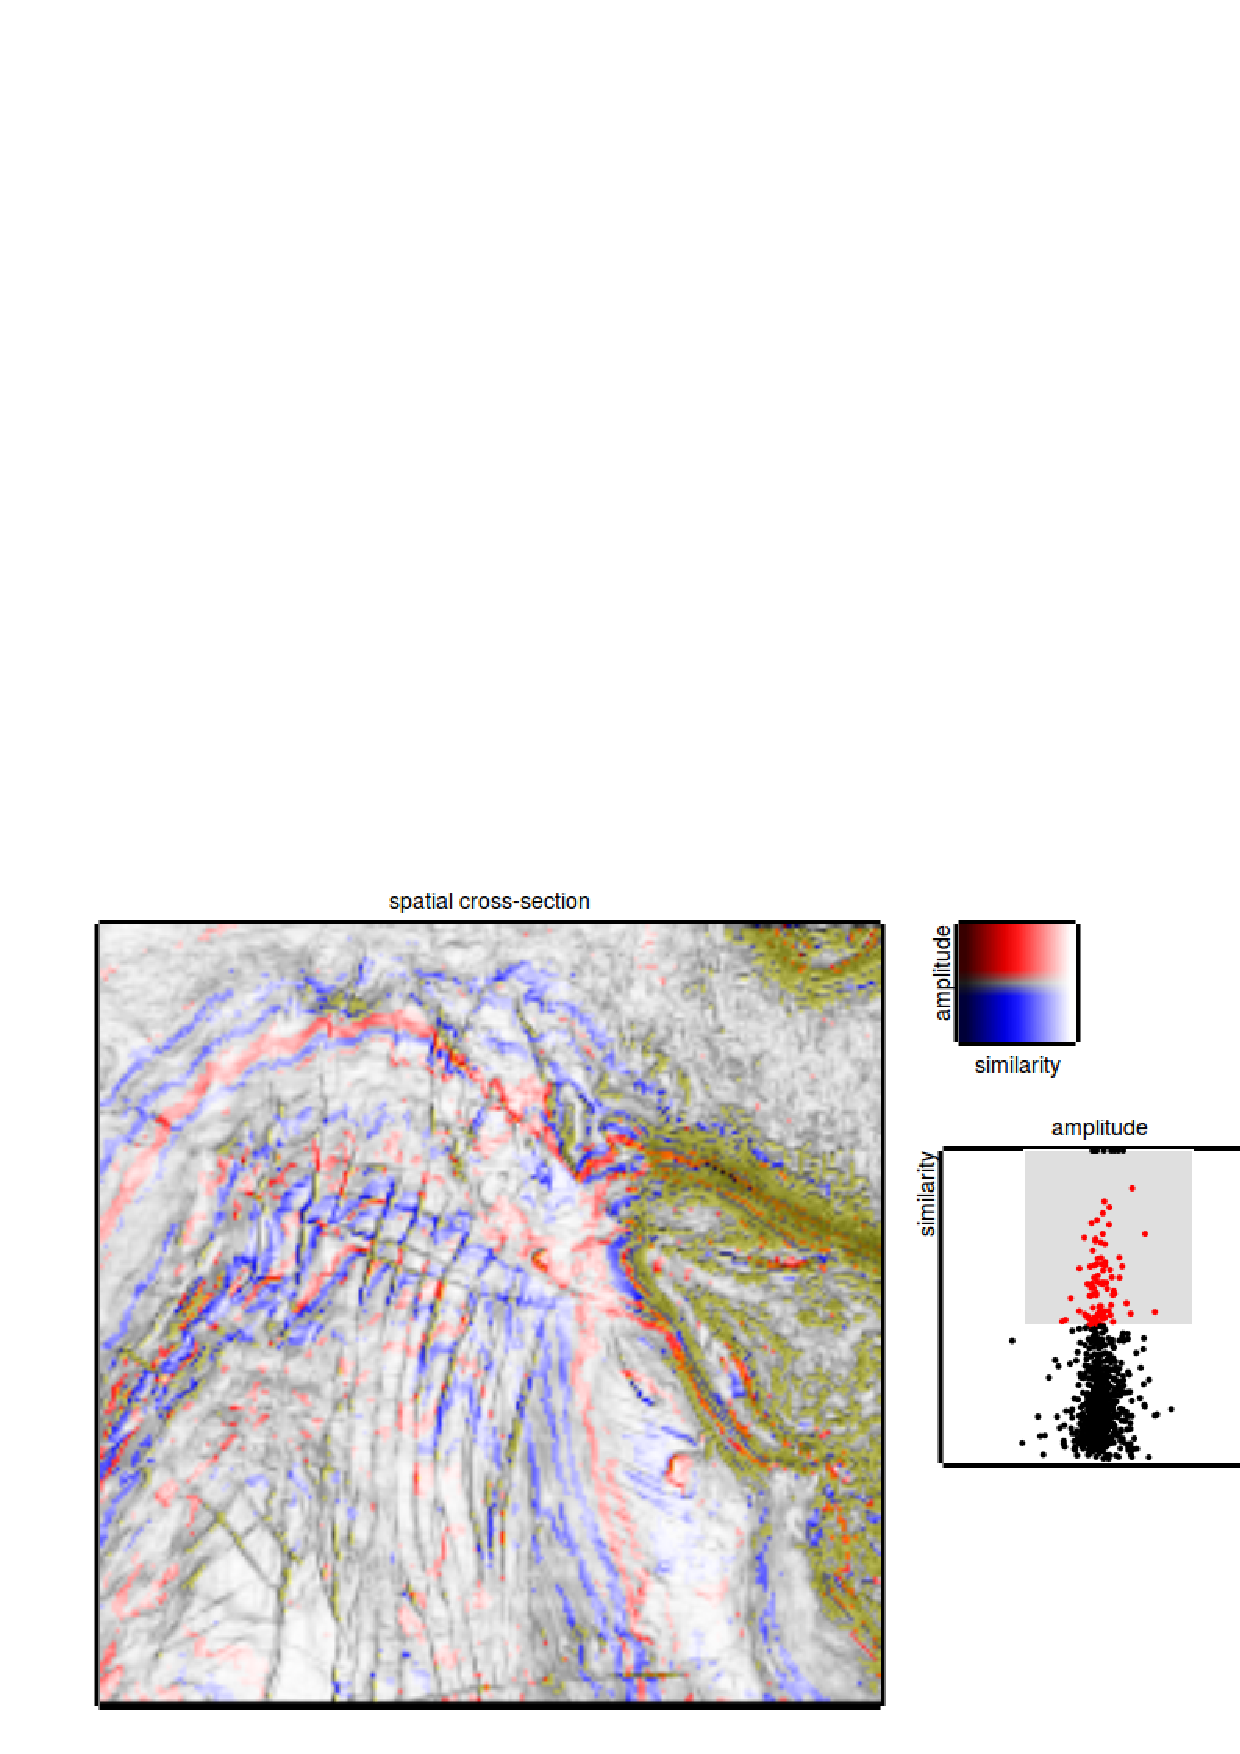
\includegraphics[width=16cm]{full_view}
  \caption{Geophyzviz: Interactive attribute analysis.}
  }

%% Uncomment below to disable the manuscript note
%\renewcommand{\manuscriptnotetxt}{}

%% Copyright space is enabled by default as required by guidelines.
%% It is disabled by the 'review' option or via the following command:
% \nocopyrightspace

%%%%%%%%%%%%%%%%%%%%%%%%%%%%%%%%%%%%%%%%%%%%%%%%%%%%%%%%%%%%%%%%
%%%%%%%%%%%%%%%%%%%%%% START OF THE PAPER %%%%%%%%%%%%%%%%%%%%%%
%%%%%%%%%%%%%%%%%%%%%%%%%%%%%%%%%%%%%%%%%%%%%%%%%%%%%%%%%%%%%%%%%

\begin{document}

%% The ``\maketitle'' command must be the first command after the
%% ``\begin{document}'' command. It prepares and prints the title block.

%% the only exception to this rule is the \firstsection command
\firstsection{Introduction}

\maketitle

%% \section{Introduction} %for journal use above \firstsection{..} instead

In exploration geophysics, analysts relate anomalies in seismic data to
potential targets of interest such as reservoirs and gas contacts.
Seismic data is typically acquired by firing an impulsive source into the earth and
recording the reflected energy at receivers at the surface, as shown in Figure \ref{seismic_acq}. The reflection data creates an image
of the subsurface of the earth called a seismic image. Reflections are caused by
impedance contrasts between sedimentary layers of the earth, where the impedance is a function
of the physical properties of the materials at the interface. 
\begin{figure}[htb]
\centering
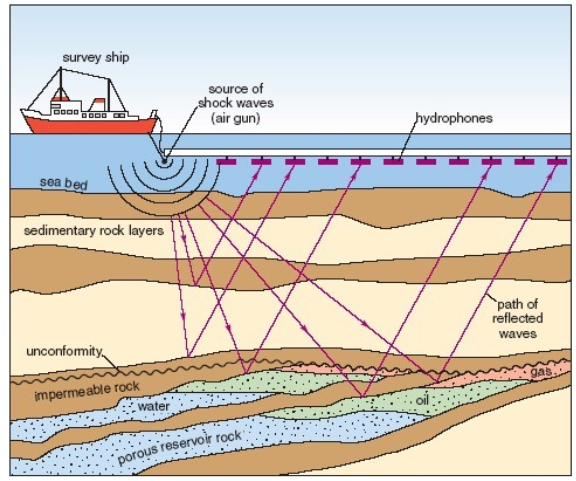
\includegraphics[width=3in]{seismic}
\caption{Seismic data acquisition.}
\label{seismic_acq}
\end{figure}

Each reflection appears in the data as
a scaled, filtered, and modulated copy of the source waveform. The goal of quantitative
seismic interpretation is to relate the shape of the reflected waveform to physical
properties of the reflection interface. Unfortunately the transfer function is grossly
undetermined which forces analysts to use indirect methods in order to classify reflections.

\begin{figure}[htb]
\centering
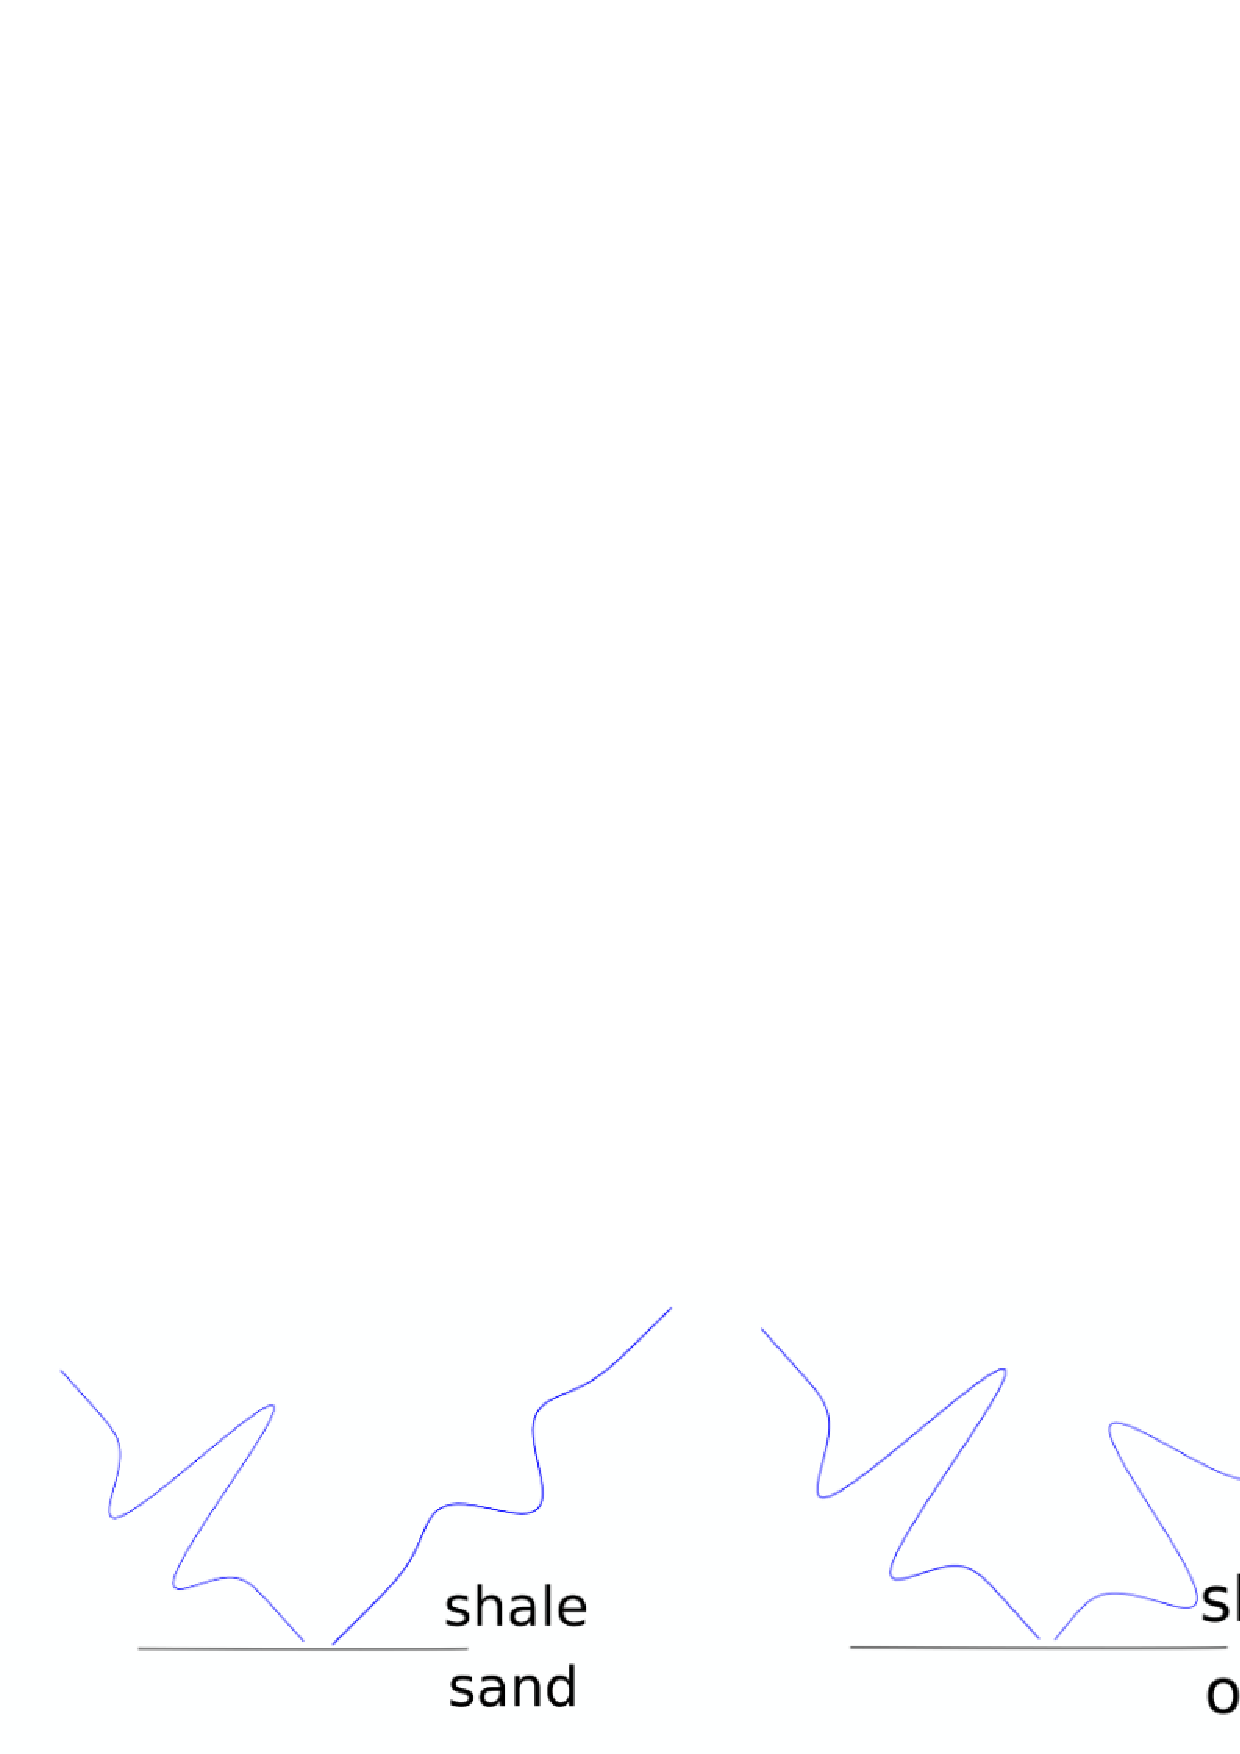
\includegraphics[width=3in]{signal_analysis}
\caption{Example of a reflected waveform changing shape at an interface of geological contrasts.}
\label{analysis}
\end{figure}

A seismic attribute can loosely be defined as a quantity derived from seismic data
that can be analyzed in order to enhance information that might be more subtle
in a traditional seismic image \ref{wiki:attr}. The zoo of specific seismic attributes is large and
outside the scope of this paper, so I will refer to seismic attributes in the general sense
of derived data. Each attribute adds a dimension to the seismic image, where every geospatial
point in the seismic image now contains a vector of derived attributes. The attributes form
a multivariate space, where analysts try to relate trends, anomalies, and clusters to
rock classifications and geospatial regions of interest.

The main workhorse for attribute analysis are cross plots, where analysts visually inspect
2D scatter plots of attributes for a chosen section of data. Points that form interesting clusters
are then geospatially cross-referenced to see if the cluster corresponds to a geospatial region in the seismic image.
This work flow is often pieced together using disparate software packages for geospatial visualization
and statistical analysis. Data extraction and reformatting is often required to move between applications
and rudimentary tools such as side-by-side screen shots are unfortunately used for analysis.
Expensive commercial software packages offer some integrated options, but these packages are not general
purpose or lack the interactivity required to efficiently visualize the data space.

Geophyzviz provides a visualization driven approach to seismic attribute analysis. I integrate
scatter plots and geospatial displays as interactive linked views in the same application to allow
analysts to quickly explore for data anomalies and seamlessly cross-reference the anomalies to geospatial
regions. I increase the information density of the seismic image by using a bi-variate colour map to
co-render two attributes, and generalize the tool by providing cross plots and co-rendered images of
every combination of attributes. An overview display facets the the entire multivariate data set into
scatter plot matrices and juxtaposed small multiples of co-rendered seismic images. I use slow animated
transitions which encourages the user to visually track how clusters and points move through
the multivariate data space. Finally, brushes are used to interactively select and highlight
points on the scatter plot, which are then superimposed on the seismic image to allow to for
instant geospatial cross-referencing. Geophyzviz is hosted as an open-source project on github
and currently serving as a public facing web-app at http://www.geophyzviz.appspot.com.



\section{Previous work}


There are several existing commercial software packages for seismic attribute analysis, the
two most popular being Schlumberger's Petrel and CGG's Hampson-Russel. Both these packages
focus on two specific attributes and do not generalize to the entire multivariate attribute space.
Viewing geospatial referencing of attributes is poorly linked to the actual seismic image and requires
generating and loading new data sets. The software has nested menus and controls for navigation
which requires the analyst to switch focus from the data. The work-flow for analyzing two attributes
using Petrel is documented in the tutorial video \cite{petrel-vid}, which can serve as a benchmark for user experience.

The idea to co-render attributes in the seismic image was inspired by a blog post by Evan Bianco \cite{bianco-2015}, but is
also documented in the geophysical literature \cite{chopra-attr}. Each seismic attribute is designed to exploit different
properties, for example similarity will highlight faults and fractures while the attenuation (Q) attribute
can indicate the presence of a fluid. Co-rendering two attributes can aid in delineating structure and facies
in a seismic image.

The literature on seismic attribute visualization is sparse, but there has been much work in
generalized multivariate visualization. Burger and Hauser \cite{fuchs-vom-2009} provide an overview of the current
state of the art and describe a general set of tools for effective visualization of multivariate data. In addition to
an abstract pipeline for scientific visualization, the authors suggest the following general approaches:
Derivations, glyphs, hybrid/multi-method visualization, interaction, layering and fusion, two level rendering, 
n-D viewing, probing, reduction, machine learning. Not all of these approaches are valid for seismic interpretation,
but the design of Geophyzviz is heavily based on this framework. Seismic attributes themselves are already derivations,
and the dimensionality of the dataset does not require abstraction to level of glyphs. Hybrid/multimethod visualization
is the application of several visualization techniques to the same image, which I apply by displaying the same seismic image 
created from different seismic attributes. Geophyzviz is highly interactive, which is described as the most important tool
for understanding complex data. I use interactive summary views for data navigation, animated transitions for the movement
between detail views, and selection brushes that link multiple diplays. I make use of layering and fusion by combining two attributes
into a bivariate colour map and superimposing selected targets in a semi-transparent layer. Multiple views encourage comparison and
can give contrast to help generate correct understanding. I make heavy use multiple views by faceting the entire the multivariate
dataset in overview displays consisting of small multiples. Although not currently implemented in Geophyzviz, larger seismic datasets will
likely require probing, where a smaller subset of the data can be isolated based on user selection. A machine learning approaches
to seismic attribute visualization are discussed in the Future work section.


Seismic attribute analysis is closely linked to hyper-spectral imaging, as they both involve
analysis of high dimensional geospatial data. The commercial software package ENVI \cite{itt-sol} by
exelisvis provides hyper-spectral visualization and automated image segmentation, while
packages Gerbil \cite{gerbil} and MultiSpec \cite{multispec} provide open-source options. Ideas on general visualization
and interactivity can borrowed from the hyper-spectral community, however there are fundamental
differences between hyper-spectral images and seismic attributes. Hyper-spectral data is considered
to be multidimensional, where the spectral bands are analyzed independently from each other.
Classifications are made directly on the spectral curves corresponding to each pixel. Seismic
attributes on the other hand are multivariate, where interpretation requires analysis of
relationships between attributes. In addition to display a multidimensional image, geophyzviz
also needs to display multivariate information between attributes.


\begin{table}
%% Table captions on top in journal version
 \caption{Data abstraction}
 \label{data_abstract}
 \scriptsize
 \begin{center}
   \begin{tabular}{cccc}
     Year & Submitted & Accepted & Accepted (\%)\\
   \hline
     1994 &  91 & 41 & 45.1\\
     1995 & 102 & 41 & 40.2\\
     1996 & 101 & 43 & 42.6\\
     1997 & 117 & 44 & 37.6\\
     1998 & 118 & 50 & 42.4\\
     1999 & 129 & 47 & 36.4\\
     2000 & 151 & 52 & 34.4\\
     2001 & 152 & 51 & 33.6\\
     2002 & 172 & 58 & 33.7\\
     2003 & 192 & 63 & 32.8\\
     2004 & 167 & 46 & 27.6\\
     2005 & 268 & 88 & 32.8\\
     2006 & 228 & 63 & 27.6
   \end{tabular}
 \end{center}
\end{table}


\section{Data abstraction}

Seismic data is generated by using an impulsive source to create a wavefield in the Earth,
which is sampled by a grid of receivers at the surface. Each receiver records 1D timeseries data called a trace,
which is measurement of reflected energy vs depth at a given spatial position. The collection of traces
form a seismic volume, where cross-sections through the volume are called seismic images. A seismic
image can reveal structure about where reflection interfaces are, but more information is required
to determine physical properties about the Earth. The seismic volume is processed to create seismic
attributes, which are the same dimension as the seismic volume. Attributes
can themselves be plotted as an image, or plotted against each other as crossplots. Patterns
and trends in crossplots can be heuristically linked to physical properties of the Earth.

\begin{figure}[htb]
\centering
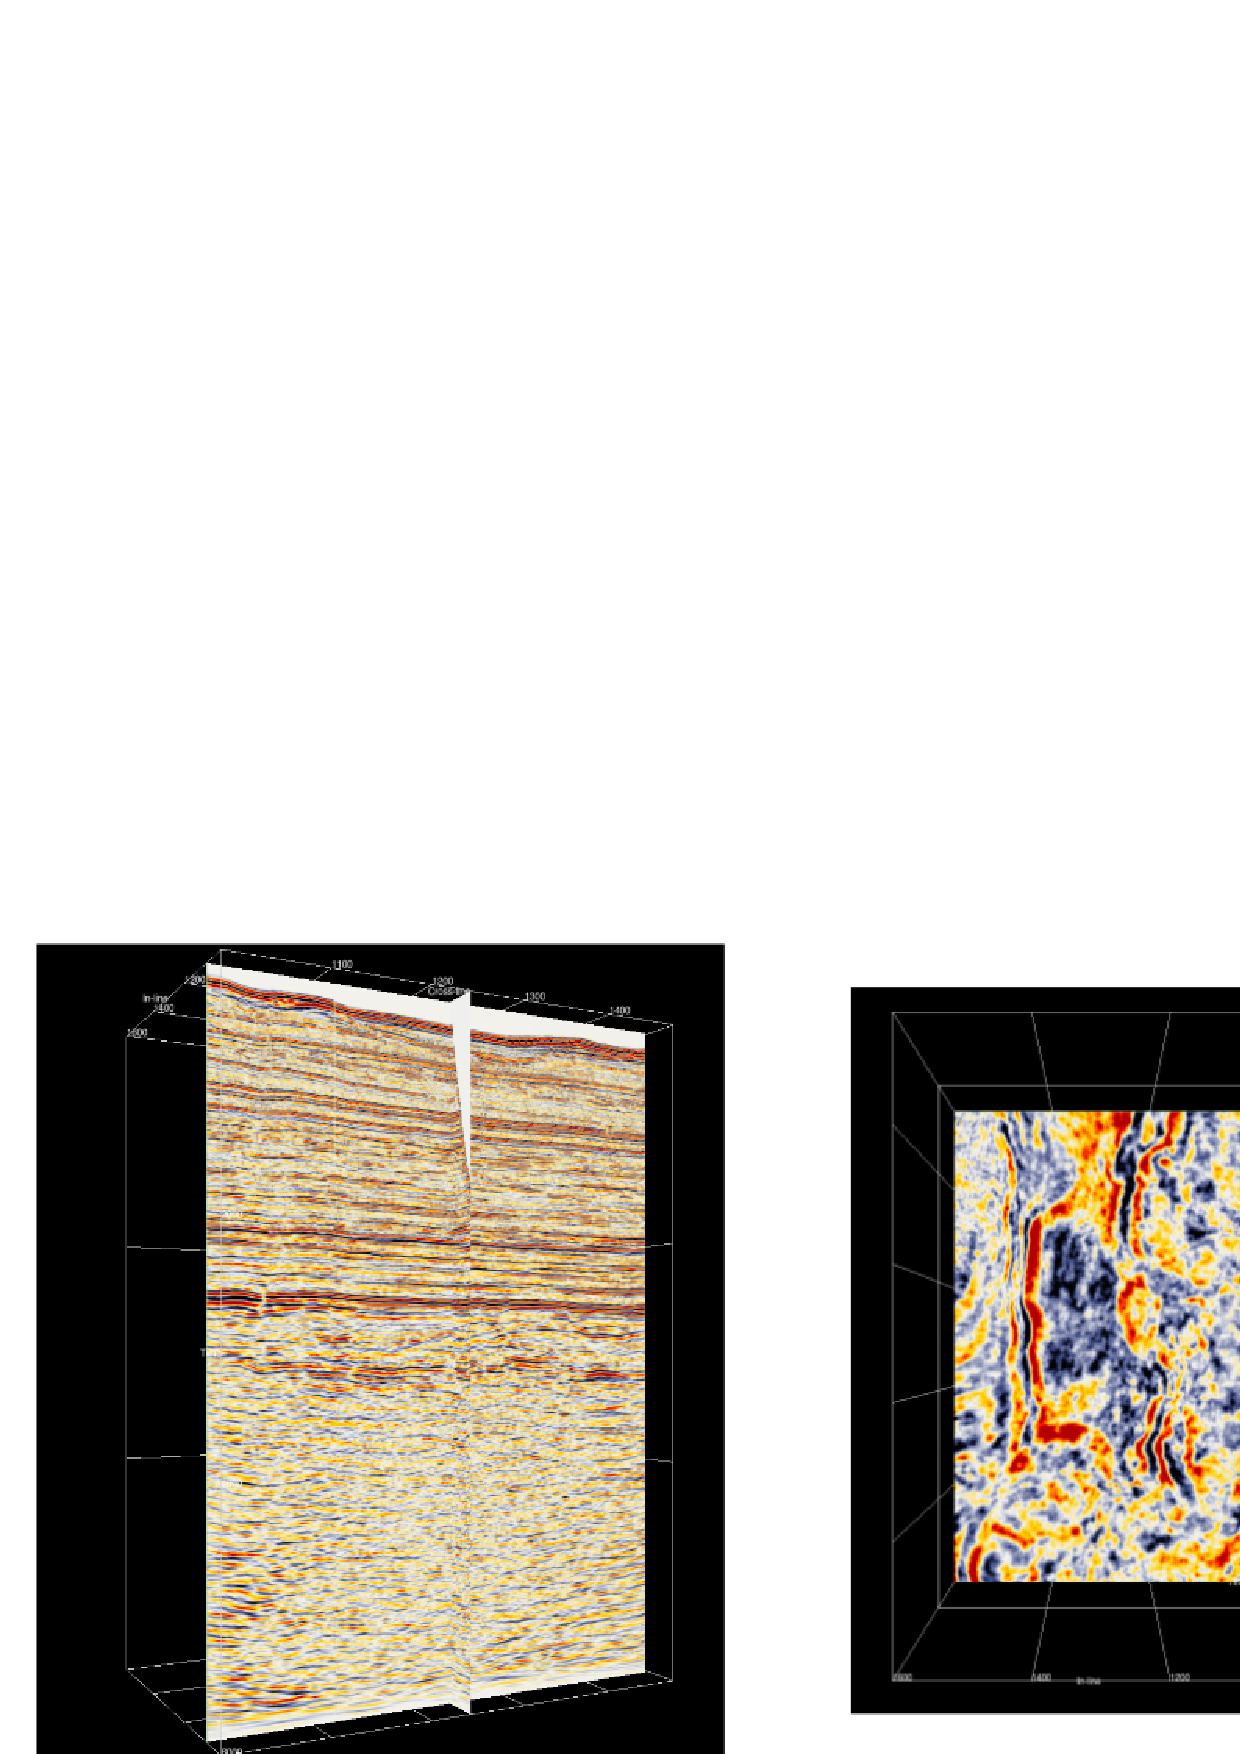
\includegraphics[width=3in]{seismic_slices}
\caption{Seismic data acquisition.}
\label{seismic_acq}
\end{figure}

Abstractly, seismic data is a 3D static spatial scalarfield where each cell corresponds to the reflected energy at a latitude, longitude, and depth. 
Seismic attributes are derived from the seismic data, and the full seismic attribute dataset form a multivariate 3D tensor 
field where each cell contains the derived seismic attribute values. Analysis is performed on a 2D cross-section of the attribute dataset,
which is a 2D multivariate tensor field. When seismic attributes are analyzed independently of their spatial position, the dataset can be
flattened into a list of items, where each item is contains the attribute values from a given cell.


\section{Task abstraction}
The general task of seismic analysis is to find anomalous regions in seismic images
that may be an indicator resource reservoirs or something of geological interest.
Seismic images alone do not contain enough information to reveal these regions, so
seismic attributes are used to aid analysis. Multivariate analysis of attributes is 
heuristically related physical properties of the Earth, so analysts look for and compare
visual trends and anomalous clusters in attribute scatter plots. These trends and clusters
are geospatially cross-referenced to the seismic image to see if
they correspond to a region of structural interest.

\begin{figure}[htb]
\centering
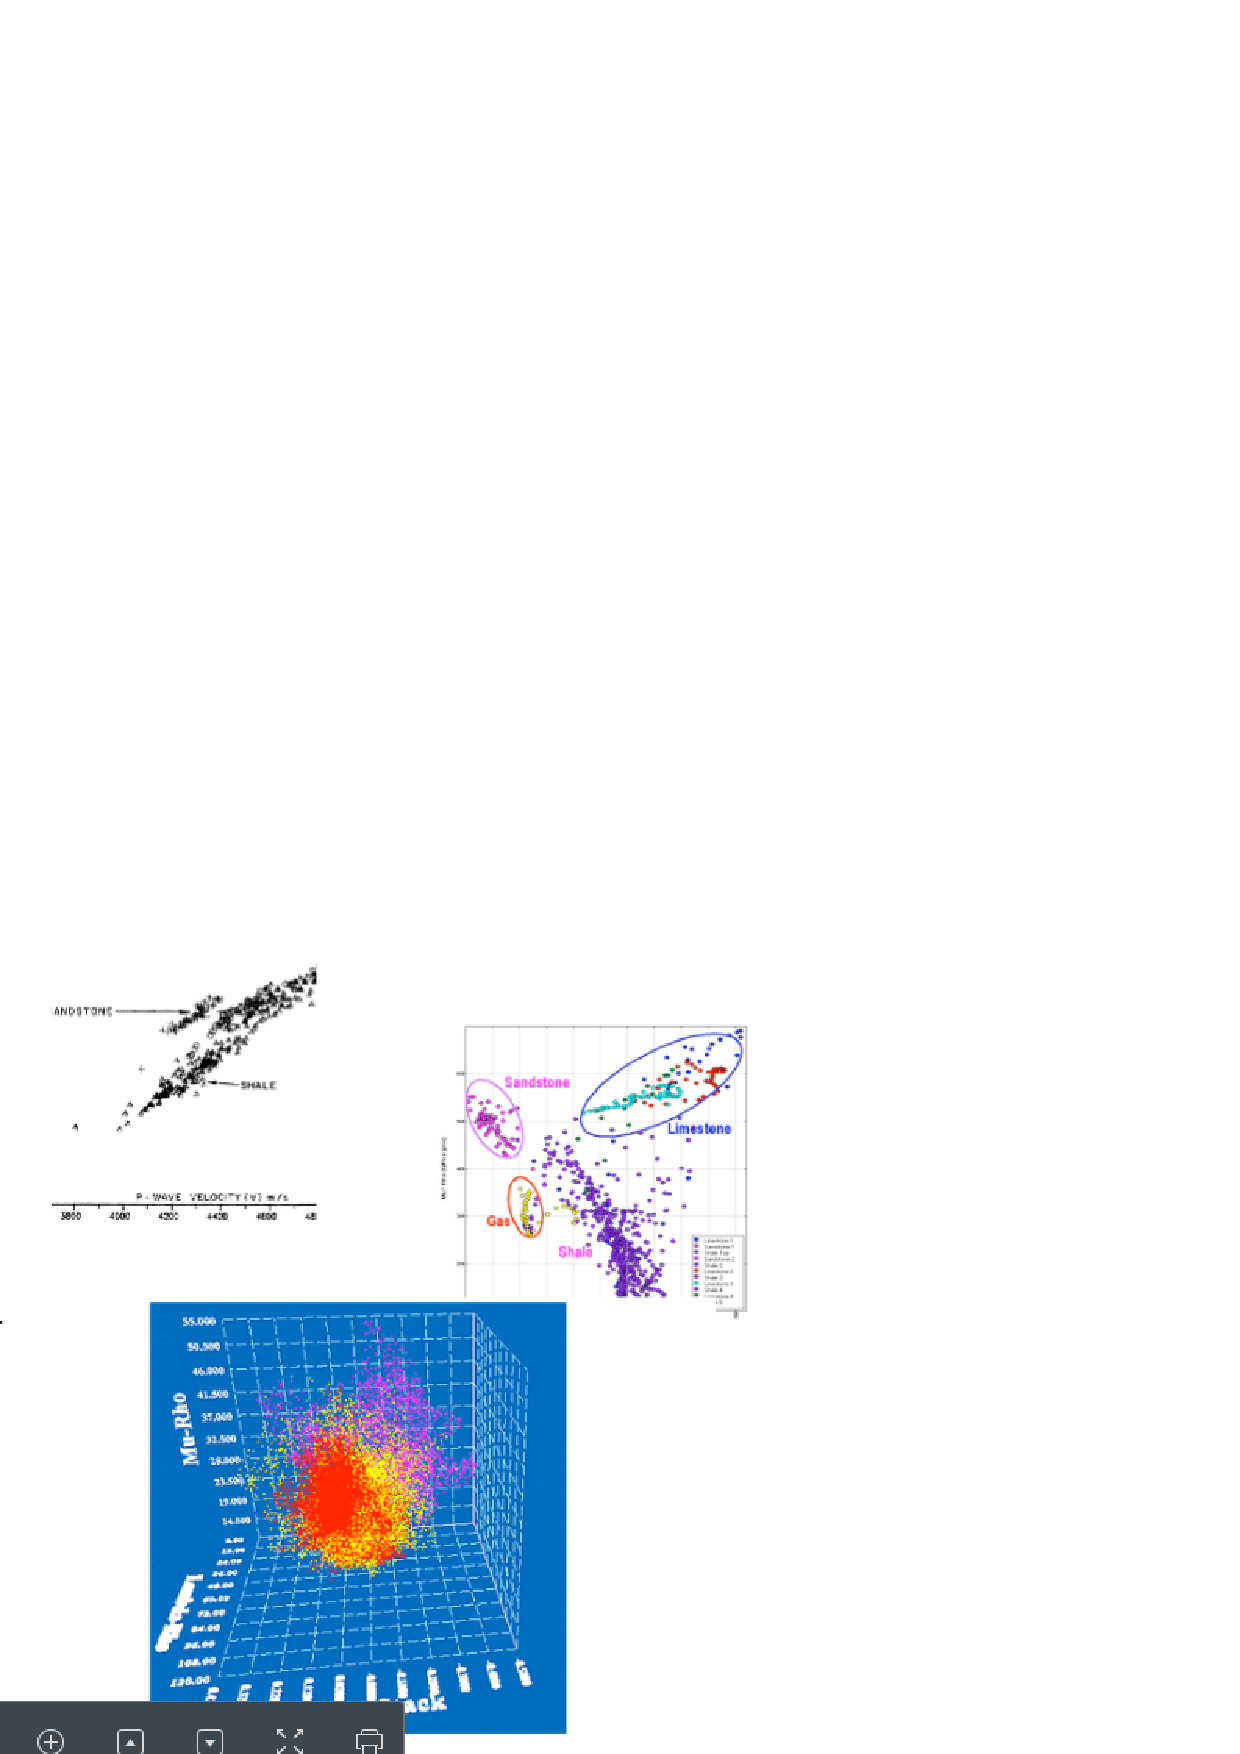
\includegraphics[width=3in]{attr_anal}
\caption{Seismic data acquisition.}
\label{seismic_acq}
\end{figure}

At the highest level, the analyst is consuming the data in order discover new information
and generate  hypothesis' from the seismic image. The targets are geospatially localized multivariate trends, anomolies, and clusters. 
Although the analyst has some a priori knowledge of patterns to search for, primarily both the type of target and location are unknown
so the analyst needs to explore the data. Once a potential targets has been identified via visual analysis of a scatter plot, the target 
is then compared to relationships in other scatter plots. The target is then summarized by viewing its geospatial structure. 

\section{Solution}
The solution focuses on integrating and interacting with five core components:
the geospatial image display, the geospatial overview, the scatter plot display,
the scatter plot overview, and the linked target selection brush. 

\subsection{Geospatial display}
Seismic images are typically displayed in variable density images, or heat maps where
the value of the grid points are mapped to the colour channel via a sequential colour map. I take
advantage of the magnitude channels saturation and lightness to optionally co-render two attributes
in the same seismic image. This information dense technique allows an analyst to directly locate
correlations and similarities between two attributes in one view. I form the co-rendered image from
a simple HSL blending algorithm which generates an HSL array from a primary attribute,
and modulates the lightness channel by the amplitude of a secondary attribute.
For attributes that are +/-, I use a diverging colourmap that moves from blue to white to red for the hues, 
and use a sequential colourmap with green hues for magnitude data. I do not render images with +/- data as secondary 
attributes as the lightness channel is magnitude only.

\begin{figure}[htb]
\centering
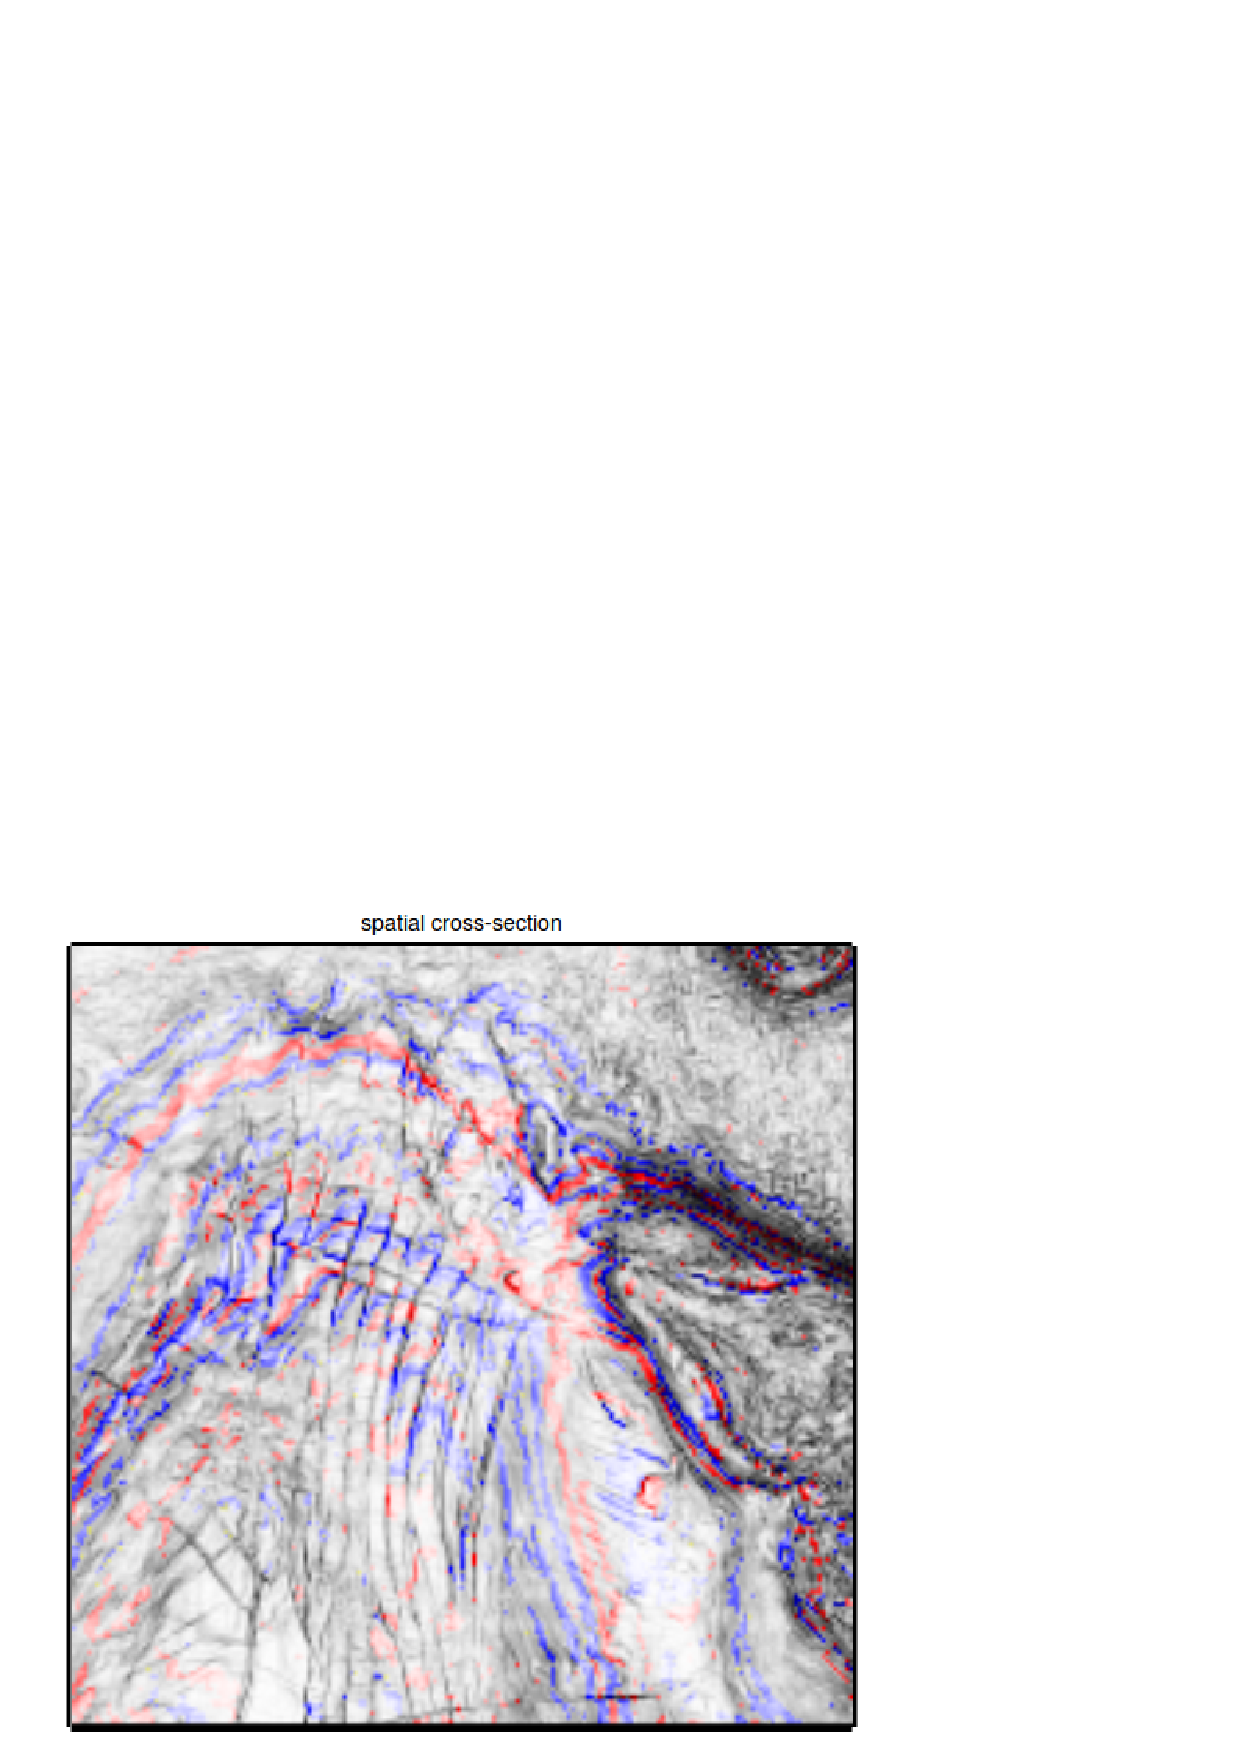
\includegraphics[width=3in]{corender}
\caption{The spatial cross-section view with amplitude and similarity attributes co-rendered using a bivariate colour map.}
\label{spatial_plot}
\end{figure}

\subsection{Geospatial overview}
The content of the geospatial display is controlled by the geospatial overview panel, which facets every corendering
possiblilty into a matrix of small multiples. The geospatial overview serves the purpose of data navigation 
as clicking on a small multiple will update the focus of the geospatial display. Geophyzviz is built without 
control panels and menus and uses the data itself as the interface whenever possible. In addition to navigation,
the juxtaposed small multiples in the geospatial overview serve as analysis view; the analyst is encouraged to
look for contrasts between images. The diagonal column of the matrix is univariate data with one attribute
plotted in greyscale. The centre row corresponds to amplitude data as the secondary attribute, which is left
deliberately blank +/- data does not map well the lightness magnitude channel.

\begin{figure}[htb]
\centering
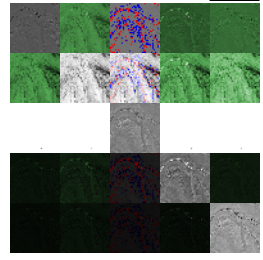
\includegraphics[width=3in]{corender_overview}
\caption{The overview panel for attribute correndering views.}
\label{overview_space}
\end{figure}

\subsection{Scatterplot display}
The scatter plot display spatially encodes the attribute values in order to visualize targets
consisting of trends, correlations, outliers, and clusters. The scatter plot is typically a focal
point of the attribute analysis workflow and is therefore positioned in the centre of the visualization.
As the analyst navigates to another set of attributes, slow transitions are deliberately used to encourage
the analyst to track a target as it moves through the multivariate space. The choice of using 2-D scatterplots
is to avoid occlusion and avoid ambiguity when using selection brushes. 

\begin{figure}[htb]
\centering
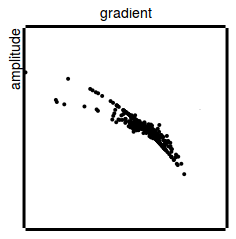
\includegraphics[width=3in]{crossplot}
\caption{Detail view of a scatter plot of intercept and amplitude attributes.}
\end{figure}

\subsection{Scatterplot overview}
The number of attributes in a seismic dataset is typically <12, so the entire multivariate scatterplot space
can visualized in a scatterplot matrix. Similiar to the geospatial overview, I use the scatterplot overview
data as the navigation interface for changing the focus of the scatterplot display. The scatterplot matrix also
serves as an analysis tool by allowing contrast comparisons.

\begin{figure}[htb]
\centering
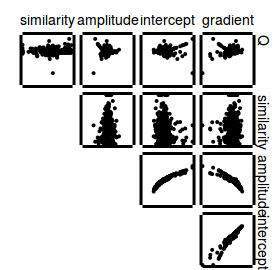
\includegraphics[width=3in]{scatterplot_matrix}
\caption{Scatterplot matrix of overviewing all attribute combinations.}
\end{figure}

\subsection{Target selection brush}
All of the views are linked via an interactive selection brush. Analysts use a brush to
select a target on the scatter plot view. This highlights the target points in each cell of the 
scatterplot overview, which encourages side by side comparisons. The brush also links to the geospatial display,
where the selected targets are superimposed as a semi-transparent mask allowing for instant
geospatial referencing and target summary. 

\begin{figure}[htb]
\centering
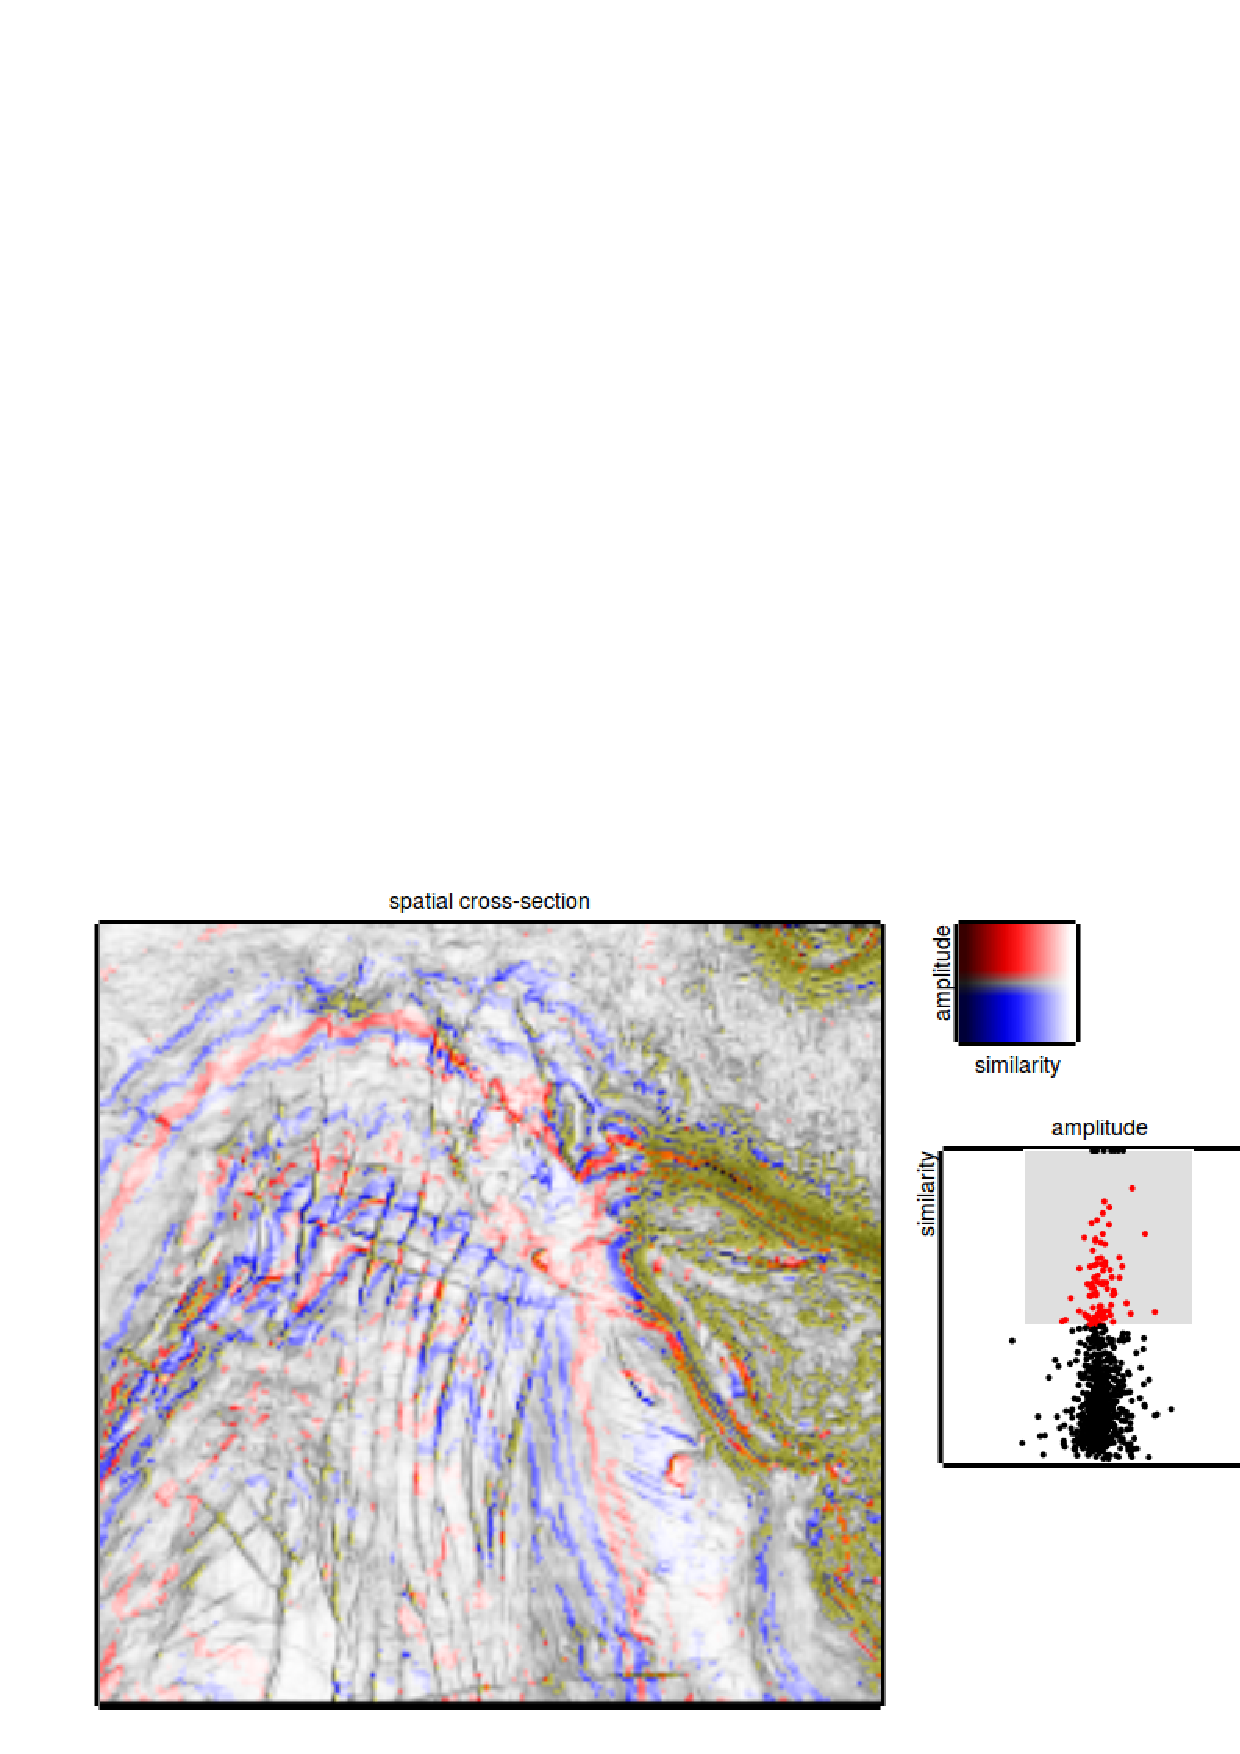
\includegraphics[width=3in]{full_view}
\caption{Using the target selection brush to highlight a target on multiple plots.}
\end{figure}

\section{Implementation}
Geophyzviz is developed as a web application where data processing and formatting
is handled on a cloud-hosted back-end server and visualizations are generated
on the client's browser. I chose to use the webapp paradigm as analysts can use and demo the tool without downloading
and building any software. The back-end data server is written in Python and the visualization
is built on top of the D3 charting library in JavaScript.

The back-end is relatively simple, and primarily handles data requests from the client and
basic pre-processing such as normalization, image down-sampling for the small multiples, and array masking
for the superimposed image. I used the webapp2 framework for url routing and Google App Engine as 
a cloud host.

The client side visualization code uses the html5 canvas for image plots and 
d3 data bindings to SVG elements for the scatter plots.  Interactivity
drives AJAX calls to back-end to dynamically update the client-side data. The angularJS framework was used as the
client-side architecture.

The source code is open-source and hosted on GitHub.

\section{Results}
I demonstrate the prototype application with the open F3 seismic data set collected offshore New
Zealand. The data was processed for amplitude and coherency attributes, while intercept,
gradient, and attenuation (Q) attributes were synthesized for the demonstration.

The typical scenario is an analyst trying to find geologically interesting regions and form
a hypothesis based on analysis of seismic attributes. Starting from
the initial view, the analyst will scan the overview plots and compare the images looking
for features to pop out. Once they notice something of interest, they click on the
small plot to bring the data into the detail view. At this point the analysts will spend
time free playing, switching between detail views and watching how points rearrange
themselves through the multivariate attribute space. Once they have explored the space
searching for targets of trends, features, outliers, and clusters, they can query a target
using the interactive selection brush. Selecting a target on the scatter plot immediately highlights
the affected points on the plots the in the scatter matrix. The analyst can then compare
the juxtaposed plots to see if the selected target also forms trends in other scatter plot
views. Once a target has been analyzed in the multivariate scatter plots, the analyst
will focus their attention on the image plot. The selection brush is linked to the
image plot, where points from the selected target are superimposed as a semi-transparent
mask. Ideally a valid target will form a geologically relevant shape on the image plot.
The analysts can then explore attribute co-rendering options by clicking on the small multiple
images. If a target pops out on particular attribute co-rendering views, the analyst
can make an interpretation about the geological significance of the target.


\section{Discussion and future work}
I applied principals of information visualization to address a broken
work-flow is exploration geophysics. I developed an integrated and interactive
approach to seismic attribute analysis which used linked views and faceted small
multiples to let analysts explore the multi-dimensional, mutlivariate data space.

The greatest strength is the information density and interactivity of the display. The overview 
of juxtaposed small multiples allows the user to see the entire multivariate data space
in one view. The interactivity allows the analyst to quickly focus on targets to form and
test hypothesis. The interactivity is data-driven, so the analyst can change views and make
selections by clicking and the selecting the data rather using controls outside the visualization. 
The data as interface design choice lets the user focus on the data analysis task without having switch
to a control panel to change the view.

The data chosen for the demonstration was a manageable size, but interactive scatter plot
displays will be a challenge with larger data sets. The d3 charting library provides easy methods for
interacting with svg elements, but this approach quickly becomes inefficient as the number of
points becomes large. For larger seismic images a more efficient plotting approach using low-level
graphics card libraries like openGL or webGL will be a necessity. Additional approaches to embedding
data and down-sampling may be required to display larger seismic images.

Choosing adequate colour maps for each possible co-rendering is another difficult challenge
that has not been fully addressed. I made simple design choices of colour maps, where I normalized
data and used diverging and sequential maps where reasonable. Attributes have a large spread of
values and dynamic ranges, so each combination of co-rendering requires attention to colour map detail.
The current implementation has some very effective colour maps, but others require more attention.

The biggest lesson I learned during this project is to use the data as the interface. The first iteration
of the concept consisted of only detailed views and a control panel for navigation and interaction.
Replacing the control panel with overview displays which themselves drive interactivity and navigation
greatly increased the information density of the display.

Although I designed Geophyzviz for data consumption tasks, I can extend the functionality
to include data production tasks. After the analyst has explored the data and generated hypothesis,
they may wish to create annotations and classifications of the targets. The current tool allows
selection of just one target at a time, but I can foresee many situations where an analyst would
save selections and generate a collection of multiple targets. The produced output of the tool would
would be a segmented seismic image where the segments are derived from attribute analysis. It would
relevant to perform automated clustering and let the analysts use the tool for quality assurance of
the clustering algorithm.

The focus of the design was on seismic attributes, but the application generalizes to any multidimensional
geospatial data sets. Immediate applications are hyper-spectral image analysis and remote sensing. More abstractly
the tool can be used to visualize features in image classification and segmentation problems.


\section{Conclusion}
I presented Geophyzviz, a data visualization tool for exploring multidimensional, multivariate
geospatial data. The tool was successfully demonstrated on the F3 seismic data set and received
general positive feedback from geophysical interpreters. Although useful for small data sets., future work is required to scale to scatter plots of many points. 


\bibliographystyle{abbrv}
%%use following if all content of bibtex file should be shown
%\nocite{*}
\bibliography{template}
\end{document}
